%System Design

\chapter{Impementation}
In this chapter we describe the framework and application implementation. We refer to the technologies we used and their interaction. In some cases we cite some crucial code chunks and explain them. Initially we describe the REST API and we analyze its contents. After an extensive illustration of the back end tier of the framework, we emphasize in the front end. There we mention the technologies that are used and their implementation. Alongside the front end description, we present some fragments of front end use cases.

\section{General JavaScript practices and patterns}
\begin{figure}
	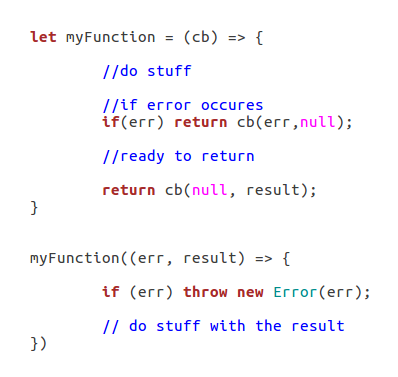
\includegraphics[scale=0.7]{cb.png}
	\caption{Example of a callback function}
	\label{cb}
\end{figure} 
In the framework we developed, we make use of javascript in both front and back end. This programming language uses asynchronous logic, which takes place through the usage of asynchronous callback functions. A callback function is a method which receives as an argument another method, in order to call it later. The execution of the first function does not block the execution of the rest of the program commands. When the execution of the first function ends, the execution of the callback function begins. An example of a callback function can be seen in figure ~\ref{cb}. \par
	In our framework, the callback functions are used constantly, thus the design and implementation are transformed accordingly. As a convention, all the callback functions receive as arguments two objects, the error and the result. Before the execution of the callback function, in case an error occures, the execution stops and the error object is passed to the callback. The result object is obviously null. If no errors occure, the error object is null and the result object contains the function outcome. Next we describe two design patterns, which are based in callback functions and are heavily used in the framework implementation.

\subsection{Closures}
\begin{figure}
	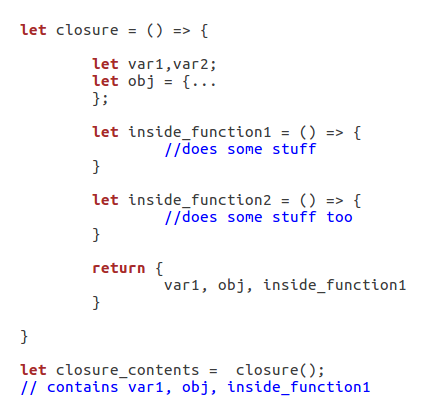
\includegraphics[scale=0.7]{closure.png}
	\caption{Example of a closure function}
	\label{closure}
\end{figure} 
Javascript is an object oriented language and is created to perform well in any platform. Thus, it has many ways of defining certain structures, such as classes. In our framework, we define our classes through the closure design pattern. Closures fully implement a class functionality.\par
	Genarally, a closure in javascript is a function. This function receives arguments that initialize its state. The function body defines its contents, such as variables, objects and other functions. In the end the function returns, or exposes in the rest of the framework, only what is necessary. This may include also variables, objects and functions. Everything that is not returned, equals to what classes define as private. An example of this pattern is shown in figure ~\ref{closure}.

\subsection{Thunks}
\begin{figure}
	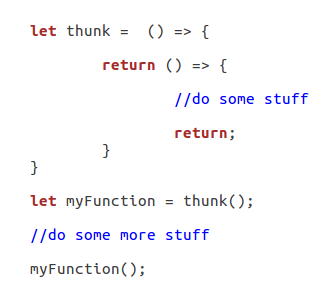
\includegraphics[scale=0.7]{thunk.png}
	\caption{Example of a thunk function}
	\label{thunk}
\end{figure} 
The thunk pattern has a similar structure with closure, but its used in a different way. Basically, its a function which returns another function. The intersting part is that the execution of the first function does not imply the execution of the second. This way we define lazy functions, meaning methods which are scheduled to execute, but they are not until they have to. This pattern is important for solving a problem that occures in javascript, known as callback hell. This problem takes place due to the generation of large sequence of nested callback functions, which is considered a bad design practice and creates debug problems. An example of the thunk pattern is shown in figure ~\ref{thunk}.

\section{Back-End implementation}
In this section we focus in the back end implementation of the framework. Initially we present the REST API and then we describe the development stages of the framework modules. We emphasize in the technologies used and their in between communication.

\subsection{REST API}
An important part of the back end framework implementation is the development of the rest api, which is achieved through routing.Routing refers to determining how an application responds to a client request for a specific endpoint, which is a URI (or path) and a specific HTTP request method (GET, POST, PUT or DELETE). Each of our routes has different route handler functions, which are executed when the route is matched. The route handler functions use the information, which is given to them through the request, and after the execution of internal operations, return a response object to the client.\par
	 The response object has a concrete structure and includes all the required information. Among other things, it contains the status code and the result data. Generally the content of the response object is determined from the request method and the success of the operation (errorHandling is described thoroughly in chapter FDHJKSAJFJKASDJKJFAS). The structure of the response object is in JSON format. \par 
	 	Next we present all the routes for each model entity seperately. For some of them we describe their corresponding handlers.
	 	
\paragraph{}
The routes of the table ~\ref{authURI} are used from the framework for the authentication of the users. The login route checks whether the client's credential exist in the users model of the database. If the client is identified, a positive confirmation is sent to the user, while at the same time a session cookie is saved (session management is described in chapter FDHJSAFAS). In opposite case, the server's response is negative. The logout route disconnects the user from the framework and its corresponding session cookie is deleted from the database. The last route is used from the framework to check if the user is already authenticated. If this event occures, the authentication operation is skipped.

\paragraph{Users}

In table ~\ref{usersURI} are presented the routes which concern the users model. The POST method is responsible for the creation of new user instances. It checks whether all fields have a value and the username and email properties are unique. The figure TADE presents the structure of a User instance. The GET method returns the user instance information and the project, in which he participates. The PUT and DELETE methods are used for their corresponding functionalities.


\paragraph{Projects}




\begin{table}[]
\centering
\begin{tabular}{|c|c|}
\hline
\rowcolor[HTML]{32CB00} 
\textbf{URI}     & \textbf{method} \\ \hline
\rowcolor[HTML]{FFFFFF} 
/login           & GET             \\ \hline
\rowcolor[HTML]{67FD9A} 
/logout          & GET             \\ \hline
\rowcolor[HTML]{FFFFFF} 
/isauthenticated & GET             \\ \hline
\end{tabular}
\caption{Authentication URI's}
\label{authURI}
\end{table}


\begin{table}[]
\centering
\begin{tabular}{|c|c|c|}
\hline
\rowcolor[HTML]{32CB00} 
\textbf{Model} & \textbf{URI}                                                     & \textbf{method}                                     \\ \hline
\rowcolor[HTML]{FFFFFF} 
Users          & /users/?id=\{user\_id\}                                              & GET                                                 \\ \hline
\rowcolor[HTML]{67FD9A} 
Users          & /register                                                        & POST                                                \\ \hline
\rowcolor[HTML]{FFFFFF} 
Users          & /users/?id=\{user\_id\}                                              & PUT                                                 \\ \hline
\rowcolor[HTML]{67FD9A} 
Users          & \multicolumn{1}{l|}{\cellcolor[HTML]{67FD9A}/users/?id=\{user\_id\}} & \multicolumn{1}{l|}{\cellcolor[HTML]{67FD9A}DELETE} \\ \hline
\end{tabular}
\caption{Users URI's}
\label{usersURI}
\end{table}



\begin{table}[]
\centering
\begin{tabular}{|c|c|c|}
\hline
\rowcolor[HTML]{32CB00} 
\textbf{Model} & \textbf{URI}                   & \textbf{method} \\ \hline
\rowcolor[HTML]{FFFFFF} 
Projects       & /projects/?id=\{project\_id\}      & GET             \\ \hline
\rowcolor[HTML]{67FD9A} 
Projects       & /projects                      & POST            \\ \hline
\rowcolor[HTML]{FFFFFF} 
Projects       & /projects/join/?id=\{project\_id\} & GET             \\ \hline
\end{tabular}
\caption{Projects URI's}
\label{projectsURI}
\end{table}


\begin{table}[]
\centering
\begin{tabular}{|c|c|c|}
\hline
\rowcolor[HTML]{32CB00} 
\textbf{Model}                                         & \textbf{URI}                                                               & \textbf{method}                                     \\ \hline
\rowcolor[HTML]{FFFFFF} 
Datasets                                               & /datasets/?id=\{dataset\_id\}                                              & GET                                                 \\ \hline
\rowcolor[HTML]{67FD9A} 
Datasets                                               & /datasets                                                                  & POST                                                \\ \hline
\rowcolor[HTML]{FFFFFF} 
Datasets                                               & /datasets/list/?id=\{dataset\_id\}                                         & GET                                                 \\ \hline
\rowcolor[HTML]{67FD9A} 
Datasets                                               & /datasets/grid/?id=\{dataset\_id\}                                         & GET                                                 \\ \hline
\rowcolor[HTML]{FFFFFF} 
\multicolumn{1}{|l|}{\cellcolor[HTML]{FFFFFF}Datasets} & \multicolumn{1}{l|}{\cellcolor[HTML]{FFFFFF}/datasets/?id=\{dataset\_id\}} & \multicolumn{1}{l|}{\cellcolor[HTML]{FFFFFF}DELETE} \\ \hline
\end{tabular}
\caption{Datasets URI's}
\label{datasetsURI}
\end{table}



\begin{table}[]
\centering
\begin{tabular}{|c|c|c|}
\hline
\rowcolor[HTML]{32CB00} 
\textbf{Model} & \textbf{URI}            & \textbf{method} \\ \hline
\rowcolor[HTML]{FFFFFF} 
Posts          & /posts/?id=\{post\_id\} & GET             \\ \hline
\rowcolor[HTML]{67FD9A} 
Posts          & /posts                  & POST            \\ \hline
\rowcolor[HTML]{FFFFFF} 
Posts          & /posts/?id=\{post\_id\} & UPDATE          \\ \hline
\rowcolor[HTML]{67FD9A} 
Posts          & /posts/?id=\{post\_id\} & DELETE          \\ \hline
\end{tabular}
\caption{Posts URI's}
\label{postsURI}
\end{table}



\begin{table}[]
\centering
\begin{tabular}{|c|c|c|}
\hline
\rowcolor[HTML]{32CB00} 
\textbf{Model} & \textbf{URI}            & \textbf{method} \\ \hline
\rowcolor[HTML]{FFFFFF} 
Plots          & /plots/?id=\{plot\_id\} & GET             \\ \hline
\rowcolor[HTML]{67FD9A} 
Plots          & /plots                  & POST            \\ \hline
\rowcolor[HTML]{FFFFFF} 
Plots          & /plots/?id=\{plot\_id\} & DELETE          \\ \hline
\end{tabular}
\caption{Plots URI's}
\label{plotsURI}
\end{table}


